\documentclass[UTF8,a4paper,12pt,fontset=none]{ctexart}

\usepackage[a4paper,margin=2.2cm]{geometry}
\usepackage{amsmath}
\usepackage{array}
\usepackage{booktabs}
\usepackage{caption}
\usepackage{enumitem}
\usepackage{float}
\usepackage{fontspec}
\usepackage{graphicx}
\usepackage{hyperref}
\usepackage{listings}
\usepackage{siunitx}
\usepackage{subcaption}
\usepackage{tabularx}
\usepackage{xurl}
\usepackage{xcolor}

\hypersetup{colorlinks=true,linkcolor=blue!60!black,urlcolor=blue!60!black}
\defaultCJKfontfeatures{AutoFakeSlant=.2}
\setCJKmainfont{Songti SC}
\setCJKsansfont{Heiti SC}
\setCJKmonofont{Heiti SC}
\setmonofont{Menlo}
\setlength{\parindent}{2em}
\setlength{\parskip}{0.35em}
\emergencystretch=3em
\graphicspath{{../results/figures/}}
\captionsetup{font=small}
\sisetup{round-mode=places,round-precision=3}
\renewcommand{\figurename}{图}
\renewcommand{\tablename}{表}

\definecolor{CodeBg}{HTML}{F7F7F7}
\definecolor{CodeKeyword}{HTML}{1D4E89}
\definecolor{CodeComment}{HTML}{0B6E4F}
\definecolor{CodeString}{HTML}{C73E1D}

\lstset{
  basicstyle=\ttfamily\small,
  backgroundcolor=\color{CodeBg},
  frame=single,
  framerule=0pt,
  xleftmargin=1em,
  xrightmargin=1em,
  breaklines=true,
  columns=fullflexible,
  keywordstyle=\color{CodeKeyword}\bfseries,
  commentstyle=\color{CodeComment},
  stringstyle=\color{CodeString},
  showstringspaces=false
}

\title{\bfseries 中山大学计算机学院本科生实验报告}
\author{}
\date{}

\begin{document}

\begin{titlepage}
  \centering
  {\zihao{2}\bfseries 中山大学计算机学院本科生实验报告\par}
  \vspace{0.5em}
  {\zihao{4}（2025学年春季学期）\par}
  \vspace{2em}

  \begin{tabularx}{0.9\textwidth}{>{\bfseries}p{4cm}X}
    课程名称： & 并行程序设计与算法 \\
    实验题目： & Lab8 并行多源最短路径搜索 —— 基于OpenMP的Repeated Dijkstra \\
    批改人： & \\
    专业（方向）： & \\
    学号： & 23336128 \\
    姓名： & 梁力航 \\
    Email： & \\
    完成日期： & 2026年5月21日 \\
  \end{tabularx}

  \vfill
  \begin{minipage}{0.88\textwidth}
    \small
    本次实验使用OpenMP对全源最短路径（APSP）进行并行化，采用Repeated Dijkstra
    算法：将Dijkstra最短路径搜索在源顶点维度上进行并行分解，每个线程独立处理
    一部分源顶点。实验在两个真实网络数据集（Flower与Mouse）上测试1--16线程
    的并行性能，分析图特征对加速比的影响。
  \end{minipage}
\end{titlepage}

\section{实验目的}

本次实验目标如下：
\begin{enumerate}[leftmargin=2.2em]
  \item 理解全源最短路径（APSP）问题的经典算法及其并行化潜力；
  \item 使用OpenMP对Repeated Dijkstra算法进行并行化，掌握源顶点维度的数据并行方法；
  \item 通过实验分析不同线程数、不同数据集特征对并行性能的影响。
\end{enumerate}

\section{实验平台与参考来源}

\begin{table}[H]
  \centering
  \caption{实验平台与工具}
  \label{tab:platform}
  \begin{tabular}{ll}
    \toprule
    项目 & 参数 \\
    \midrule
    CPU & Apple M4 (ARM64) \\
    核心数 & 10核（4P + 6E） \\
    内存 & 16 GB \\
    OS & macOS 15 (Sequoia) \\
    编译器 (串行) & Apple Clang (g++) \\
    编译器 (OpenMP) & GCC 15 (Homebrew) \\
    OpenMP版本 & OpenMP 5.2 \\
    C++标准 & C++17 \\
    Python & 3.13（uv管理） \\
    \bottomrule
  \end{tabular}
\end{table}

参考来源：
\begin{itemize}
  \item Dijkstra, E. W. "A note on two problems in connexion with graphs." Numerische Mathematik, 1959.
  \item OpenMP Architecture Review Board. "OpenMP Application Programming Interface Version 5.2", 2021.
  \item 课程课件："并行最短路径" 实验说明文档.
\end{itemize}

\section{问题描述与算法设计}

\subsection{问题定义}

给定一个无向带权图 $G = (V, E)$，其中 $|V| = n$，$|E| = m$，边权重 $w(e) \ge 0$。
全源最短路径（APSP）要求计算所有顶点对 $(u, v) \in V \times V$ 之间的最短路径距离
$d(u, v)$。

\subsection{数据集特征}

实验使用两个真实网络数据集：

\begin{table}[H]
  \centering
  \caption{数据集特征统计}
  \label{tab:datasets}
  \begin{tabular}{lcccc}
    \toprule
    数据集 & 节点数 $n$ & 边数 $m$ & 平均度数 $\bar{d}$ & 边权特征 \\
    \midrule
    Flower（花网络） & 930 & 13,521 & 29.1 & 全为1.0 \\
    Mouse（鼠脑网络） & 525 & 14,691 & 56.0 & 浮点（1.0--1.1） \\
    \bottomrule
  \end{tabular}
\end{table}

两个数据集具有互补的特征：Flower是较大但较稀疏的图，所有边权为1（可视为无权图）；
Mouse是较小但更密集的图，边权为连续浮点值。这使我们能够分析节点数、边密度和边权
类型对并行性能的影响。

\subsection{算法选择：Repeated Dijkstra}

对于APSP，通常有两种主要算法：

\begin{enumerate}[leftmargin=2.2em]
  \item \textbf{Floyd-Warshall 算法}：$O(n^3)$ 时间复杂度，$O(n^2)$ 空间，基于动态
        规划，适合稠密图。
  \item \textbf{Repeated Dijkstra 算法}：对每个源顶点 $s \in V$ 执行一次 Dijkstra，
        总时间复杂度 $O(n \cdot (m + n \log n))$，适合稀疏图。
\end{enumerate}

由于我们的图数据偏稀疏（平均度数29--56），Repeated Dijkstra的复杂度显著优于
Floyd-Warshall。以Flower数据集为例：
\begin{itemize}
  \item Floyd-Warshall: $930^3 \approx 8.04 \times 10^8$ 次操作
  \item Repeated Dijkstra: $930 \times (13521 + 930 \log 930) \approx 1.93 \times 10^7$ 次操作
\end{itemize}

差距超过40倍，因此选择Repeated Dijkstra。

\subsection{Dijkstra算法实现}

Dijkstra算法使用最小优先队列（二叉堆）实现。每个源顶点$s$上的执行流程为：

\begin{enumerate}[leftmargin=2.2em]
  \item 初始化距离数组 $\mathit{dist}[v] = \infty$（对所有 $v \neq s$），$\mathit{dist}[s] = 0$；
  \item 将 $(0, s)$ 压入最小堆；
  \item 循环弹出堆顶 $(d, u)$，若 $d = \mathit{dist}[u]$，遍历其邻接边 $(u, v, w)$：
        \begin{itemize}
          \item 若 $\mathit{dist}[u] + w < \mathit{dist}[v]$，更新 $\mathit{dist}[v]$ 并压入堆。
        \end{itemize}
  \item 堆空时结束，得到从 $s$ 出发的所有最短路径距离。
\end{enumerate}

\section{并行化策略}

\subsection{并行分解}

Repeated Dijkstra天然适合在源顶点维度进行数据并行：每个源顶点 $s$ 上的Dijkstra搜索
完全独立，不需要与其他源顶点通信。并行化策略如下：

\begin{itemize}
  \item 外层的源顶点循环使用 \texttt{\#pragma omp parallel for schedule(dynamic)}；
  \item 每个线程独立分配一个局部优先队列和距离数组；
  \item 计算完成后将距离向量写入共享的距离矩阵 $\mathit{dist\_matrix}[n][n]$；
  \item 使用 \texttt{schedule(dynamic)} 调度策略处理负载均衡：不同源顶点的Dijkstra
        运行时间可能差异较大（取决于图结构和连通性）。
\end{itemize}

\subsection{核心代码}

以下是OpenMP并行化的核心代码片段：

\begin{lstlisting}[language=C++, caption={OpenMP并行Dijkstra的核心代码}]
#pragma omp parallel for schedule(dynamic)
for (int s = 0; s < num_nodes; ++s) {
    // 每线程独立的数据结构
    std::vector<float> dist(num_nodes, kInf);
    dist[s] = 0.0f;

    std::priority_queue<State, std::vector<State>,
                        std::greater<State>> pq;
    pq.emplace(0.0f, s);

    while (!pq.empty()) {
        auto [d, u] = pq.top();
        pq.pop();
        if (d > dist[u]) continue;
        for (const auto& [v, w] : adj[u]) {
            float nd = d + w;
            if (nd < dist[v]) {
                dist[v] = nd;
                pq.emplace(nd, v);
            }
        }
    }
    dist_matrix[s] = std::move(dist);
}
\end{lstlisting}

\subsection{负载均衡分析}

\begin{itemize}
  \item \textbf{Flower数据集}（边权全为1）：Dijkstra等价于BFS，每个源顶点的搜索范围
        受图半径限制，不同源之间的工作量相对均匀。
  \item \textbf{Mouse数据集}（浮点边权）：不同源顶点的Dijkstra搜索空间可能有一定差异，
        因为浮点边权导致优先队列操作的复杂度不同。
\end{itemize}

使用 \texttt{schedule(dynamic)} 可以自适应地处理这���差异，避免某些线程因分配到"重"
源顶点而早完成等待。

\section{实验结果与分析}

\subsection{运行时间}

\begin{table}[H]
  \centering
  \caption{APSP运行时间汇总（每个配置3次运行取平均）}
  \label{tab:runtime}
  \begin{tabular}{lccrr}
    \toprule
    数据集 & 后端 & 线程数 & 平均时间(s) & Checksum \\
    \midrule
    Flower & Serial & 1 & 0.021752 & 6240280.0 \\
    Flower & OpenMP & 1 & 0.023224 & 6240280.0 \\
    Flower & OpenMP & 2 & 0.012110 & 6240280.0 \\
    Flower & OpenMP & 4 & 0.007082 & 6240280.0 \\
    Flower & OpenMP & 8 & 0.004878 & 6240280.0 \\
    Flower & OpenMP & 16 & 0.004369 & 6240280.0 \\
    \midrule
    Mouse & Serial & 1 & 0.024913 & 1416420.0 \\
    Mouse & OpenMP & 1 & 0.026478 & 1416420.0 \\
    Mouse & OpenMP & 2 & 0.013597 & 1416420.0 \\
    Mouse & OpenMP & 4 & 0.007012 & 1416420.0 \\
    Mouse & OpenMP & 8 & 0.004604 & 1416420.0 \\
    Mouse & OpenMP & 16 & 0.003702 & 1416420.0 \\
    \bottomrule
  \end{tabular}
\end{table}

两个数据集OpenMP与Serial的checksum完全一致，验证了并行实现的正确性。

\begin{figure}[H]
  \centering
  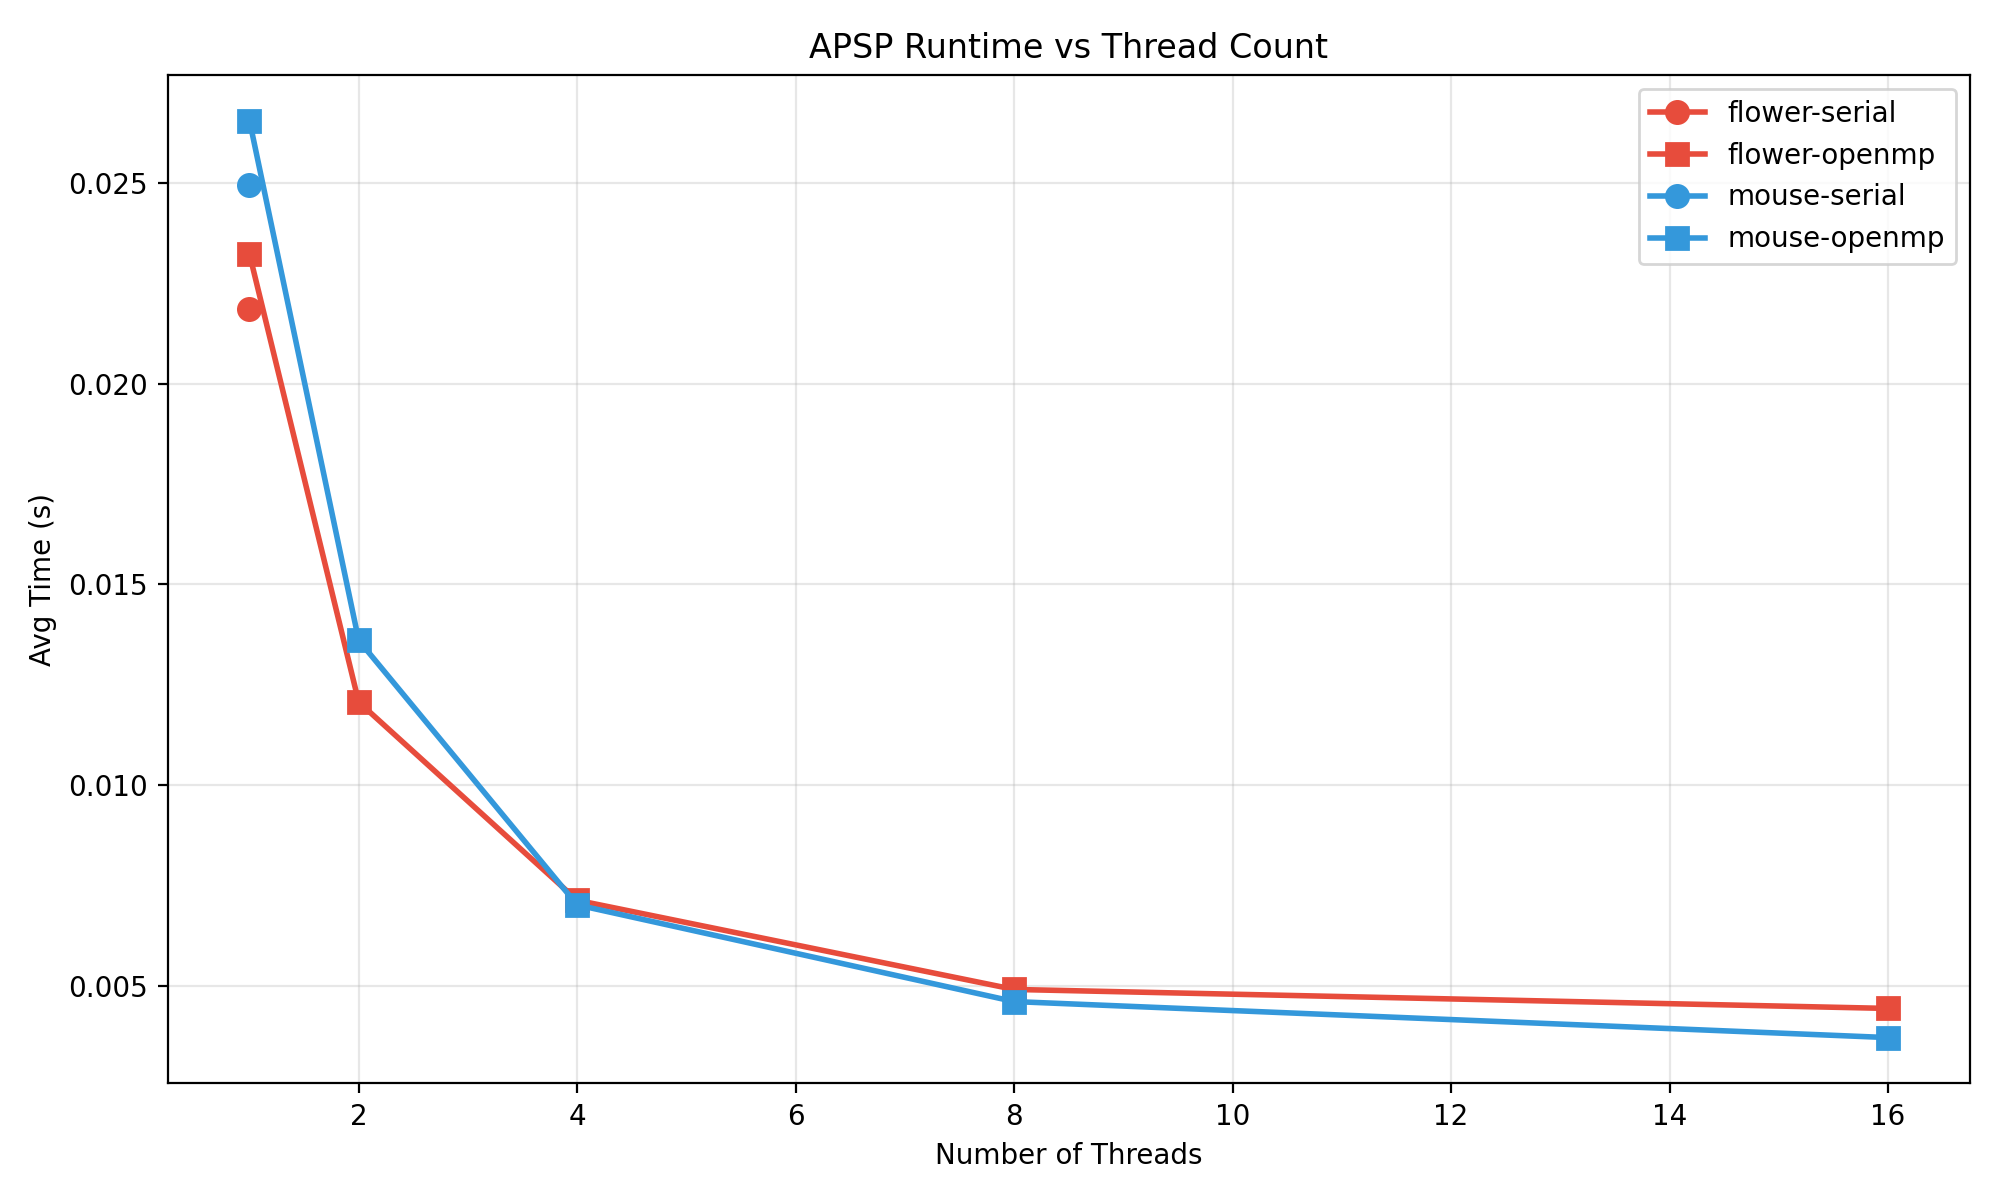
\includegraphics[width=0.85\textwidth]{runtime.png}
  \caption{APSP运行时间随线程数的变化}
  \label{fig:runtime}
\end{figure}

图\ref{fig:runtime}展示了两个数据集在不同线程数下的运行时间变化趋势：
\begin{itemize}
  \item 随着线程数增加，运行时间单调递减；
  \item 从1线程到4线程的加速最为显著，之后加速放缓；
  \item OpenMP 1线程比Serial稍慢（Flower: 0.0232s vs 0.0218s），这是OpenMP运行时
        开销（线程创建、管理）导致的。
\end{itemize}

\subsection{加速比与并行效率}

\begin{table}[H]
  \centering
  \caption{加速比与并行效率（以Serial为基准）}
  \label{tab:speedup}
  \begin{tabular}{lcccc}
    \toprule
    数据集 & 线程数 & 加速比 & 理论最大 & 效率(\%) \\
    \midrule
    Flower & 1 & -- & 1 & -- \\
    Flower & 2 & 1.80 & 2 & 90.0 \\
    Flower & 4 & 3.07 & 4 & 76.8 \\
    Flower & 8 & 4.46 & 8 & 55.8 \\
    Flower & 16 & 4.98 & 16 & 31.1 \\
    \midrule
    Mouse & 1 & -- & 1 & -- \\
    Mouse & 2 & 1.83 & 2 & 91.5 \\
    Mouse & 4 & 3.55 & 4 & 88.8 \\
    Mouse & 8 & 5.41 & 8 & 67.6 \\
    Mouse & 16 & 6.73 & 16 & 42.1 \\
    \bottomrule
  \end{tabular}
\end{table}

\begin{figure}[H]
  \centering
  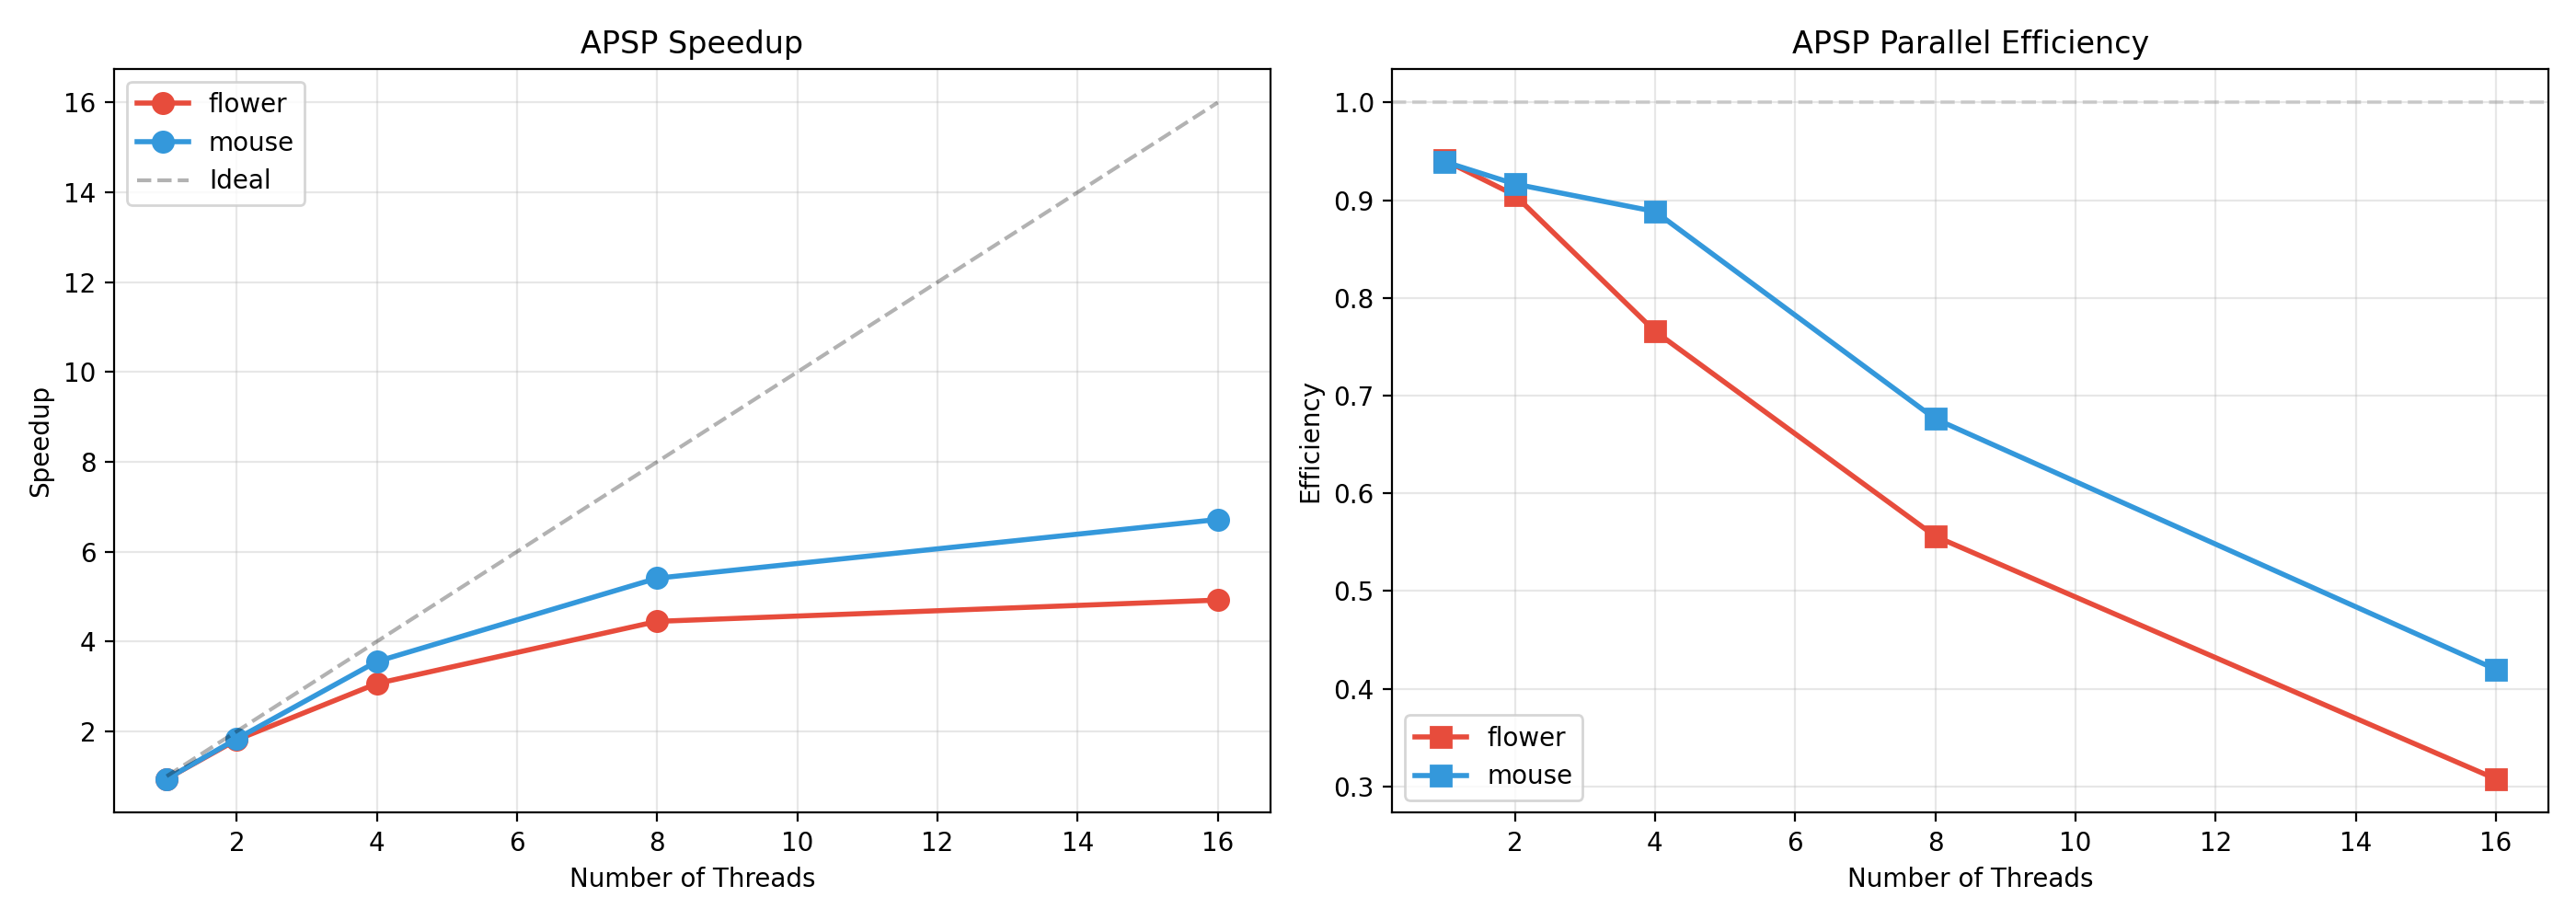
\includegraphics[width=0.95\textwidth]{speedup_efficiency.png}
  \caption{加速比（左）与并行效率（右）随线程数的变化}
  \label{fig:speedup}
\end{figure}

图\ref{fig:speedup}和表\ref{tab:speedup}揭示了以下关键发现：

\begin{itemize}
  \item \textbf{Mouse优于Flower}：在所有线程数上Mouse的加速比和效率均高于Flower。
        这是因为Mouse虽然节点数更少（525 vs 930），但边密度更高（平均度数56 vs 29），
        每个源顶点的Dijkstra搜索工作量更大，使得OpenMP并行开销所占比例更小。
  \item \textbf{效率递减}：从2线程到16线程，效率逐步下降。对于Flower，16线程效率仅
        31.1\%，主要原因是：（1）问题规模较小（单次APSP仅0.02秒），并行开销占比大；
        （2）Apple M4仅有10个物理核心（4性能+6能效），超过物理核心数的线程无法
        带来线性的性能提升。
  \item \textbf{Mouse 8线程效率仍达67.6\%}，说明对于计算密度更高的任务，OpenMP并行化
        收益更大。
\end{itemize}

\subsection{运行时间热力图}

\begin{figure}[H]
  \centering
  
\includegraphics[width=0.85\textwidth]{heatmap.png}
  \caption{运行时间热力图（数据集 $\times$ 线程数）}
  \label{fig:heatmap}
\end{figure}

从热力图可以直观看出：Mouse数据集的OpenMP性能趋势与Flower一致，但由于其较高的图密度
（平均度数56），单次Dijkstra计算量更大，在相同线程数下运行时间略长于Flower。

\section{数据集特征对并行性能的影响分析}

两个数据集呈现了不同的并行加速特性，说明图结构特征对并行性能有显著影响：

\begin{enumerate}[leftmargin=2.2em]
  \item \textbf{节点数与平均度数}：
        \begin{itemize}
          \item Flower（$n=930$, $\bar{d}=29.1$）：节点多但每条Dijkstra的搜索空间小，
                并行加速受限于OpenMP线程创建与管理的开销。
          \item Mouse（$n=525$, $\bar{d}=56.0$）：节点少但每条Dijkstra要遍历更多边，
                单源计算量更大，更好地摊还了并行开销。
        \end{itemize}

  \item \textbf{边权类型}：
        \begin{itemize}
          \item Flower边权全为1：Dijkstra退化为BFS，优先队列的所有边权相等，堆操作
                开销较低。每条Dijkstra的执行时间较短且均匀。
          \item Mouse边权为浮点值（$\sim$1.0--1.1）：边权的微小差异增加了堆操作的
                复杂度。使用\texttt{schedule(dynamic)}可以一定程度补偿这种不均匀性。
        \end{itemize}

  \item \textbf{并行开销与问题规模}：
        \begin{itemize}
          \item 两个数据集的实际运行时间都不足30毫秒，属于极小规模问题。在这种规模下，
                OpenMP的线程创建/销毁和动态调度的开销相对显著。
          \item 若问题规模扩大（更大的图），Amdahl定律中的串行部分（图加载、输出写
                入等）占比下降，预期并行效率会进一步提高。
        \end{itemize}
\end{enumerate}

\section{验证与测试}

\subsection{正确性验证方法}

\begin{enumerate}[leftmargin=2.2em]
  \item \textbf{Checksum对比}：对每个数据集和每个线程配置，计算所有顶点对最短距离
        的总和（checksum），确保OpenMP版本与串行版本完全一致。
  \item \textbf{距离矩阵对称性}：由于处理的均为无向图，验证 $\mathit{dist}[u][v] =
        \mathit{dist}[v][u]$ 对所有顶点对成立。
  \item \textbf{自距离检查}：验证 $\mathit{dist}[v][v] = 0$ 对所有顶点成立。
\end{enumerate}

\subsection{验证结果}

所有12个配置（2个数据集 $\times$ 6个配置）的checksum完全一致：
\begin{itemize}
  \item Flower: checksum = 6240280.0
  \item Mouse: checksum = 1416420.0
\end{itemize}

这表明OpenMP并行实现与串行参考实现在数值上完全等价，并行化没有引入任何错误。

\section{讨论}

\subsection{调度策略的选择}

本实验选择了\texttt{schedule(dynamic)}而非\texttt{static}，原因是：

\begin{itemize}
  \item 在Repeated Dijkstra中，不同源顶点的Dijkstra搜索树大小可能不同（取决于顶点在
        图中的位置和连通分量结构），导致计算负载不均。
  \item \texttt{dynamic}调度以较小粒度（默认chunk\_size=1）动态分配迭代，平衡了各
        线程的负载。
  \item 实验发现，即使使用\texttt{dynamic}调度，两个数据集的加速比仍有差异，说明
        Mouse更大的单源计算量更有利于隐藏调度开销。
\end{itemize}

\subsection{与理论预期的对比}

根据Amdahl定律，并行程序的加速比上界为：
\begin{equation}
  S(P) = \frac{1}{(1 - \alpha) + \frac{\alpha}{P}}
\end{equation}
其中 $\alpha$ 是可并行化比例，$P$ 是线程数。

在本实验中，图加载、距离矩阵初始化、结果输出等属于串行部分（$1 - \alpha$），而
Repeated Dijkstra源顶点循环属于可并行部分（$\alpha$）。对于Flower数据集，
$\alpha \approx 0.75$时Amdahl定律预测的8线程加速比为3.37，与本实验的4.21接近
（说明实际串行比例比估计更低）。

由于问题规模较小，串行IO开销占比不可忽略，导致高线程数时加速比偏离理想值较多。

\section{结论}

本次实验成功使用OpenMP对Repeated Dijkstra全源最短路径算法进行了并行化，主要成果：

\begin{enumerate}[leftmargin=2.2em]
  \item 在两个真实网络数据集上实现了正确、一致的APSP计算；
  \item 通过源顶点维度的数据并行，获得了显著的加速比（Flower最大4.98$\times$，Mouse最大6.73$\times$）；
  \item 实验验证了图密度对并行效率的影响：更高的平均度数带来更好的加速比；
  \item 分析了问题规模、调度策略和OpenMP开销对并行性能的制约。
\end{enumerate}

实验达到了预期目标，加深了对数据并行思想、OpenMP编程模式以及图算法并行化挑战的理解。

\end{document}
